\documentclass{article}
\usepackage[utf8]{inputenc}
\usepackage{listings}
\usepackage{xcolor}
\usepackage{float}
\usepackage{graphicx}
\usepackage{geometry}
\usepackage{array}
\usepackage{amsmath}
\usepackage{parskip}
\usepackage{enumerate}
\usepackage{hyperref}
\usepackage{caption}
\usepackage{nicefrac}

%%%%%%%%%%%%%%%%%% DO NOT TOUCH ANYTHING BELOW THIS %%%%%%%%%%%%%%%%%
\usepackage{enumitem}
\setlist[enumerate,1]{label={\alph*)}}

\usepackage{fancyhdr}
\pagestyle{fancy}
\lhead{\textbf{Computer Architecture}}
\chead{\textbf{Homework 1}}
\rhead{	
\includegraphics[width=0.2\linewidth]{fse_logo_horizontal.pdf}}

\usepackage{mdframed}

% Define the solution environment
\newmdenv[
linecolor=black,
linewidth=.5pt,
skipabove=\baselineskip,
skipbelow=\baselineskip,
innertopmargin=10pt,
innerbottommargin=10pt,
leftmargin=0pt,
rightmargin=0pt,
innerleftmargin=10pt,
innerrightmargin=10pt,
frametitle=\textbf{Solution:}
]{solution}

\definecolor{codegreen}{rgb}{0,0.6,0}
\definecolor{codegray}{rgb}{0.5,0.5,0.5}
\definecolor{codepurple}{rgb}{0.58,0,0.82}
\definecolor{backcolour}{rgb}{0.95,0.95,0.92}

\lstset{
	basicstyle=\ttfamily,
	mathescape
}
\newcolumntype{L}{>{$}l<{$}}
\newcolumntype{R}{>{$}r<{$}}
\newcolumntype{C}{>{$}c<{$}}


\title{Computer Architecture}
\makeatletter
%%%%%%%%%%%%%%%%%% DO NOT TOUCH ANYTHING ABOVE THIS %%%%%%%%%%%%%%%%%

\begin{document}
	%%%%%%%%%%%%%%%%%%%%%%%%%%%%%%%%%%%%%%%%%%%%%%%%%%%%%%%%%%%%%%%%%%%%%%%%%%%%%%%%
	%%%%%%%%%%%%%%%%%%%%%%%%%%%%%%%%%%%%%%%%%%%%%%%%%%%%%%%%%%%%%%%%%%%%%%%%%%%%%%%%
	\section*{Question 1 (4 points)}
	Convert the following decimal numbers to their 2’s complement representations (use 8 bits for each number and truncate the fractional digits if necessary):
	\begin{enumerate}
		\item $1023$
		\item $6.3$
		\item $-13$
		\item $0.04$
	\end{enumerate}
	
	\begin{solution}
	% Place your solution here
	\end{solution}
	
	
	%%%%%%%%%%%%%%%%%%%%%%%%%%%%%%%%%%%%%%%%%%%%%%%%%%%%%%%%%%%%%%%%%%%%%%%%%%%%%%%%
	%%%%%%%%%%%%%%%%%%%%%%%%%%%%%%%%%%%%%%%%%%%%%%%%%%%%%%%%%%%%%%%%%%%%%%%%%%%%%%%%
	\section*{Question 2 (6 points)}
	Perform the following operation in 2’s complement. Indicate when an overflow happens. 
	\begin{enumerate}
		\item $11001010  + 11101010$
		\item $01011010 + 00110101$
		\item $0011.1100 + 0100.0100$
		\item $11010111 - 00001011$
	\end{enumerate}
	
	\begin{solution}
		% Place your solution here
	\end{solution}
	
	
	%%%%%%%%%%%%%%%%%%%%%%%%%%%%%%%%%%%%%%%%%%%%%%%%%%%%%%%%%%%%%%%%%%%%%%%%%%%%%%%%
	%%%%%%%%%%%%%%%%%%%%%%%%%%%%%%%%%%%%%%%%%%%%%%%%%%%%%%%%%%%%%%%%%%%%%%%%%%%%%%%%
	\section*{Question 3 (10 points)}
	Write IEEE floating point representation of the following decimal numbers.
	\begin{enumerate}
		\item $19.45$
		\item $-0.028$
	\end{enumerate}
	
	\begin{solution}
		% Place your solution here
	\end{solution}
	
	
	%%%%%%%%%%%%%%%%%%%%%%%%%%%%%%%%%%%%%%%%%%%%%%%%%%%%%%%%%%%%%%%%%%%%%%%%%%%%%%%%
	%%%%%%%%%%%%%%%%%%%%%%%%%%%%%%%%%%%%%%%%%%%%%%%%%%%%%%%%%%%%%%%%%%%%%%%%%%%%%%%%
	\section*{Question 4 (10 points)}
	The following numbers are in IEEE floating point representation. Write their decimal equivalents.
		\begin{enumerate}
			\item $10111100\  11010101 \ 11100000 \ 00000000$
			\item $00000000\ 00000100 \ 00000000 \ 00000000$
	\end{enumerate}
	
	\begin{solution}
		% Place your solution here
	\end{solution}
	
	
	%%%%%%%%%%%%%%%%%%%%%%%%%%%%%%%%%%%%%%%%%%%%%%%%%%%%%%%%%%%%%%%%%%%%%%%%%%%%%%%%
	%%%%%%%%%%%%%%%%%%%%%%%%%%%%%%%%%%%%%%%%%%%%%%%%%%%%%%%%%%%%%%%%%%%%%%%%%%%%%%%%
	\section*{Question 5 (10 points)}
	Assume we are considering a set of symbols consisting of the capital English letters (26 letters) plus white-space, question mark, and full stop to communicate messages. In our coding list, the letters of the alphabet precede white-space, question mark and full stop in this representation.
	\begin{enumerate}
		\item How many bits do we need to encode each symbol in this set?
		\item Assume 32-bit words are used for communicating messages. Furthermore, assume the character codes cannot span over multiple words. Show how the following message is encoded, and what will be its equivalence in hexadecimal.
		\begin{center}
			THIS IS A SAMPLE STRING. OR IS IT?
		\end{center}
	\end{enumerate}
	
	\begin{solution}
		% Place your solution here
	\end{solution}
	
	
	%%%%%%%%%%%%%%%%%%%%%%%%%%%%%%%%%%%%%%%%%%%%%%%%%%%%%%%%%%%%%%%%%%%%%%%%%%%%%%%%
	%%%%%%%%%%%%%%%%%%%%%%%%%%%%%%%%%%%%%%%%%%%%%%%%%%%%%%%%%%%%%%%%%%%%%%%%%%%%%%%%
	\section*{Question 6 (10 points)}
	Consider the following circuit, depicted in Figure~\ref{fig:hw1-q6}. What is its output for the following inputs?
	\begin{enumerate}
		\item $a_1 a_2 = 10$,  $b_1 b_2= 11$
		\item $a_1 a_2 = 01$,   $b_1 b_2 = 00$
	\end{enumerate}
	Moreover, what does the circuit do? 
	\begin{figure}[H]
		\centering
		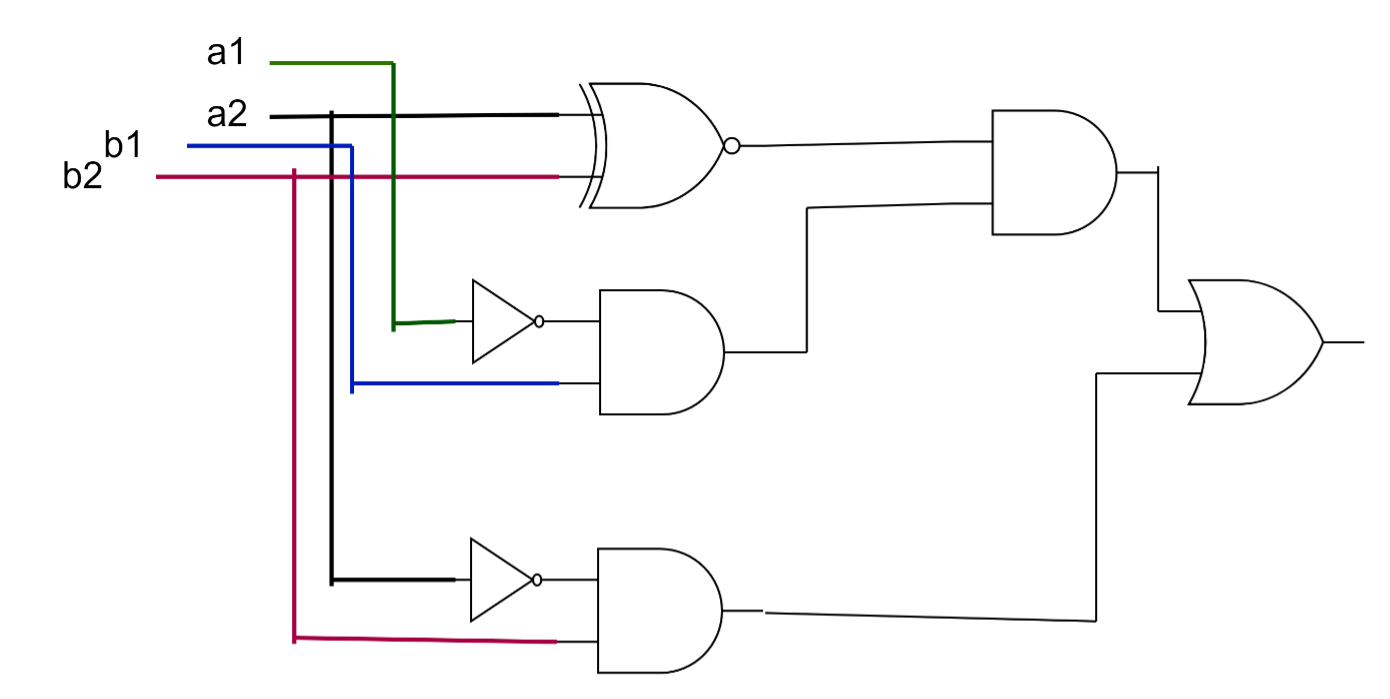
\includegraphics[width=0.7\linewidth]{./images/hw1-q6}
		\caption{}
		\label{fig:hw1-q6}
	\end{figure}
	
	\begin{solution}
		% Place your solution here
	\end{solution}
	%%%%%%%%%%%%%%%%%%%%%%%%%%%%%%%%%%%%%%%%%%%%%%%%%%%%%%%%%%%%%%%%%%%%%%%%%%%%%%%%
	%%%%%%%%%%%%%%%%%%%%%%%%%%%%%%%%%%%%%%%%%%%%%%%%%%%%%%%%%%%%%%%%%%%%%%%%%%%%%%%%
	\section*{Question 7 (10 points)}
	Design a combinational logic circuit to compare two 2-bit numbers. The output should be 0 if the numbers are not equal, and 1 if they are equal.

	\begin{solution}
		% Place your solution here
	\end{solution}
	
	
	%%%%%%%%%%%%%%%%%%%%%%%%%%%%%%%%%%%%%%%%%%%%%%%%%%%%%%%%%%%%%%%%%%%%%%%%%%%%%%%%
	%%%%%%%%%%%%%%%%%%%%%%%%%%%%%%%%%%%%%%%%%%%%%%%%%%%%%%%%%%%%%%%%%%%%%%%%%%%%%%%%
	\section*{Question 8 (10 points)}
	Using a decoder and an encoder design a circular incrementor circuit for 4-bit positive binary numbers. The input (a number between 0 and 7) will be incremented by one if its is less than 7. If the input is 7, the output should be zero.
	
	
	\begin{solution}
		% Place your solution here
	\end{solution}
	
	%%%%%%%%%%%%%%%%%%%%%%%%%%%%%%%%%%%%%%%%%%%%%%%%%%%%%%%%%%%%%%%%%%%%%%%%%%%%%%%%
	%%%%%%%%%%%%%%%%%%%%%%%%%%%%%%%%%%%%%%%%%%%%%%%%%%%%%%%%%%%%%%%%%%%%%%%%%%%%%%%%
	\section*{Question 9 (15 points)}
	We want to design a circuit to detect if an 8-bit positive binary number is divisible by 5 or not. Use a multiplexer and any necessary logic gates to design your circuit. Justify your solution.
	
	
	\begin{solution}
		% Place your solution here
	\end{solution}
	
	%%%%%%%%%%%%%%%%%%%%%%%%%%%%%%%%%%%%%%%%%%%%%%%%%%%%%%%%%%%%%%%%%%%%%%%%%%%%%%%%
	%%%%%%%%%%%%%%%%%%%%%%%%%%%%%%%%%%%%%%%%%%%%%%%%%%%%%%%%%%%%%%%%%%%%%%%%%%%%%%%%
	\section*{Question 10 (15 points)}
	Adding two numbers represented in scientific notation requires shifting floating points to make exponents equal before adding the fractions. Consider the following example:
	\begin{align*}
		1.34\cdot 10^3 &+ 2.1\cdot 10^{-1}
	\intertext{First, shift the decimal point of the smaller number to equalize the exponents:}
	1.34\cdot 10^3 &+ 0.00021 \cdot 10^3
	\intertext{Then add the fractions, and normalize the result if necessary.}
	1.34021 &\cdot 10^3
	\end{align*}
	Follow the procedure described above to add the following numbers:
	\begin{align*}
		N=14.25, \quad M=0.5
	\end{align*}
	\begin{enumerate}
		\item Convert the numbers to IEEE floating point format.
		\item Add the numbers.
		\item Normalize the result to put it in IEEE format again.
	\end{enumerate}
	
	\begin{solution}
		% Place your solution here
	\end{solution}

\end{document}